\section{Design}

The CLAS12 Trigger System was designed as a 3-stage pipeline-style system with total latency up to 8~$mu$s. Input information for the Trigger System comes from two sources:  Flash Analog to Digital Converters (FADCs) used in the photomultiplier tube (PMT)-based detectors, and Drift Chamber Readout Boards (DCRBs) used in Drift Chambers. The FADCs and DCRBs work as the pre-trigger level, reporting information to the Trigger System in the appropriate form. Stage 1 receives information from the FADCs and DCRBs and performs data processing according to the type of detector. Stage 2 performs a timing and geometry coincidence between different subsets of detectors in six groups, corresponding to the six-sector CLAS12 detector structure, as well as requires coincidence with information from central detectors. Stage 3 forms the final trigger decision. The CLAS12 Trigger diagram is shown in Fig.~\ref{fig:TriggerDiagram}.

\begin{figure}[hbt]
	\centering
	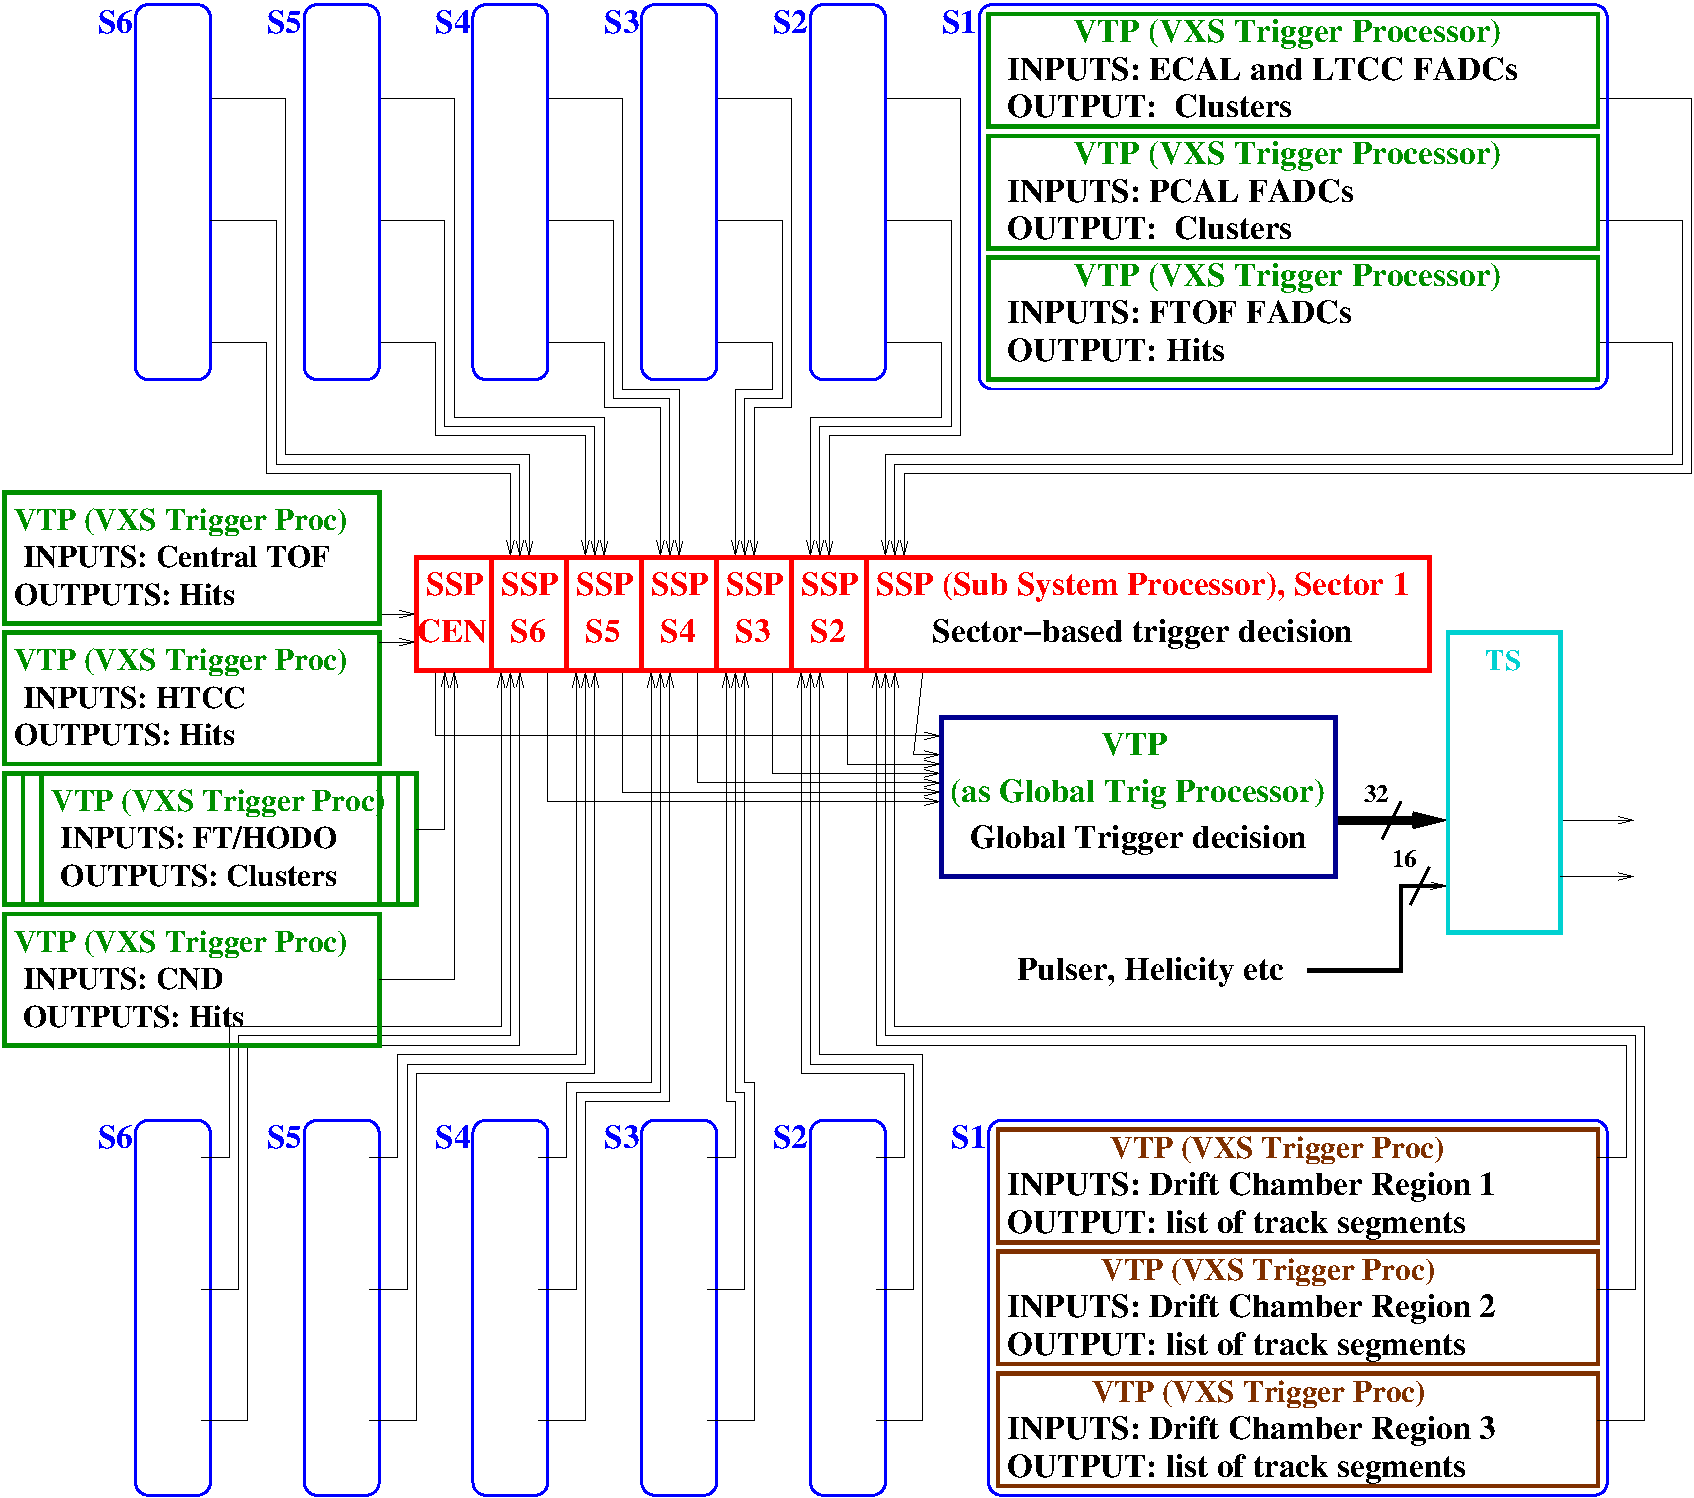
\includegraphics[width=1.0\columnwidth,keepaspectratio]{img/CLAS12_TRIGGER_1.pdf}
	\caption{The CLAS12 Trigger System diagram.}
	\label{fig:TriggerDiagram}
\end{figure}


\subsection{FADCs as Pre-trigger}

All PMT-based detectors in CLAS12 participating in the Trigger System use JLab VXS 250~MHz flash ADCs as the starting point of the trigger logic (FADC, \ref). Each channel of the FADC boards is pre-programmed with gain, pedestal, and amplitude threshold above pedestal. Every pulse above amplitude threshold is integrated and sent to the corresponding section of the Stage 1 trigger logic. The 16-channel FADC boards report 13-bit pulse integrals and 3-bit pulse time every 32~ns, which allows the following trigger logic to restore 4~ns pulse resolution while the double pulse resolution remains 32~ns. Based on the FADC reporting schedule, the following trigger logic stages can work on a 250~MHz clock, although in that case we found it problematic to meet the Field Programmable Gate Array (FPGA) timing. Because of that, our Stage 1 algorithms run on 125~MHz or slower clocks as described below. Tteh trigger information is provided to the following stages using VXS backplane serial lines.


\subsection{DCRBs as Pre-trigger}

The Drift Chamber-based trigger uses JLab 125~MHz discriminator/TDC boards (DCRB, \ref) to feed the Trigger System. These 96-channel units report hits above the pre-programmed thresholds every 16 ns. As for the FADC boards, the DCRBs are implemented in VXS format and provide trigger information using VXS backplane serial lines.


\subsection{Stage 1 Trigger} 

The Stage 1 trigger uses specially designed VXS Trigger Processor boards (VTP, see \ref). The VTP boards are installed in switch slots in every VXS crate participating in the Trigger System. The VTPs collect trigger data from the pre-trigger boards (FADCs and DCRBs) over VXS serial lines.

The most complex processing is performed for the electromagnetic calorimeters (cluster finding) and the Drift Chambers (segment and road finding). In the following sections we describe the design of the various trigger components.


\subsubsection{Electromagnetic Calorimeters}
\label{sec:ECAL}

The CLAS12 electromagnetic calorimeter (ECAL, \ref) includes two eparate subsystems, the EC and PCAL. Each consists of multiple layers of scintillating strips and lead sheets with photomultiplier readout on one side of the scintillators (the PCAL is shown in Fig.~\ref{fig:PCAL}, the EC is similar). The primary purpose of these detectors is electron identification by defining the energy and coordinate of their electromagnetic showers, referred to as clusters. The cluster finding algorithm was well established during off-line data processing development, and was adopted for the trigger implementation with some simplifications.

The algorithm first searches for one-dimensional clusters in each of the three calorimeter views (u,v,w), sorting them by energy and keeping only those above threshold, with a maximum number of four clusters in each view. Next the algorithm searches for two-dimensional clusters looking for overlap between the three views. For all two-dimension clusters found, it performs attenuation corrections based on pre-loaded tables of the attenuantion lengths of the scintillation strips using the distance from the cluster to the PMT, to deternime the correct cluster energy. Finally, the algorithm sorts the two-dimension clusters by energy and reports those above threshold, with a maximum number limited to four. For every cluster, the energy and coordinates are reported to the Stage 2 trigger every 8~ns. There is a persistency parameter that allows the same clusters to be reported for several consecutive 8~ns intervals to check for a timing coincidence with the other trigger components, as well as a timing delay parameter for the same purpose. One event with a single cluster is shown in the PCAL (preshower calorimeter) in Fig.~\ref{fig:PCAL}. The corrected energies are shown for the individual strips.

It should be mentioned that such an algorithm is designed to find clusters with a maximum energy to target electron identification. For some CLAS12 experiments, it is necessary to identify minimum-ionizing particles (MIPs) using the same trigger component. For that purpose, clusters with energy below a certain defined threshold can be selected. Such a method works for events where the number of clusters does not exceed four, otherwise there is a risk of losing low-energy clusters corresponding to MIPs. Intensive trigger efficiency studies were conducted for such cases, and the MIP trigger efficiency was measured and found acceptable.

\begin{figure}[htp]
	\begin{center}
		\centering
		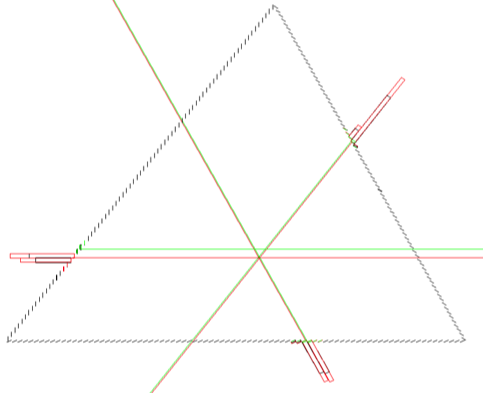
\includegraphics[width=7cm]{img/pcal1.png}
		%\includegraphics{PCA.pdf}
		\caption{Trigger System representation of a cluster reconstruction using the three views of the PCAL in one sector of CLAS12.}
		\label{fig:PCAL}
	\end{center}
\end{figure} 


\subsubsection{High Threshold Cherenkov Counter}
\label{sec:HTCC}

The CLAS12 High Threshold Cherenkov Counter (HTCC, \ref) serves as one of the primary components of the electron trigger logic. It was specially designed to discriminate electrons from other charged particles. The HTCC consists of 48 mirror sections readout by PMTs connected to FADCs (see Fig.~\ref{fig:multihitHTCC}). For trigger purposes, a 2x2 section sliding window is used to identify clusters. The cluster may include from one to four PMT signals collecting the Cherenkov light from the adjacent mirrors as shown in  Fig.~\ref{fig:multihitHTCC}. The configuration parameters include the single channel energy threshold, cluster multiplicity threshold, and cluster energy threshold. The results are reported to the Stage 2 trigger as 48-bit masks every 4 ns. The FADC ``gain'' configuration parameter allows for PMT energy calibrations, making it possible to set energy thresholds in terms of the number of photoelectrons.


\begin{figure}[htp]
	\begin{center}
		\centering
		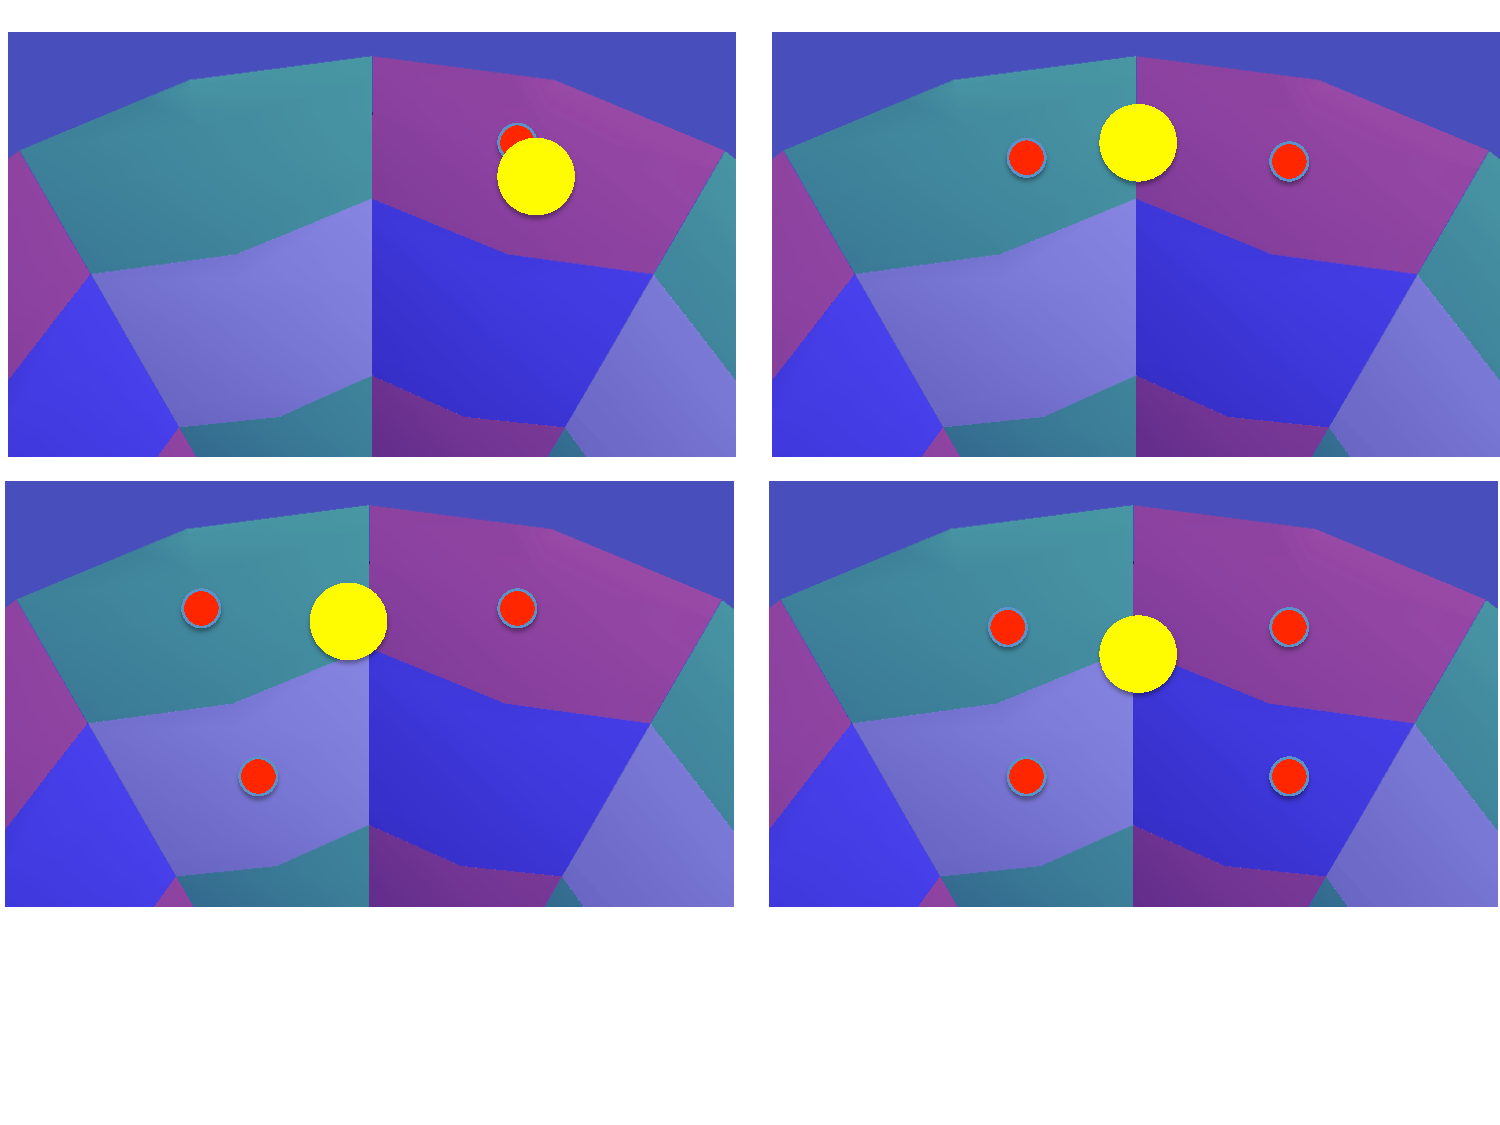
\includegraphics[width=8cm]{img/multiHits.pdf}
		\caption{Hits registered by the HTCC (red circles) and the reconstructed cluster position (yellow). The hit position and cluster position coincide for one hit clusters (top left plot), which has the lowest position resolution.}
		\label{fig:multihitHTCC}
	\end{center}
\end{figure} 


\subsubsection{Drift Chamber}
\label{sec:DC}

The CLAS12 Drift Chambers (DC, \ref) contain six superlayers in each of the six CLAS12 sectors. Each superlayer contains six layers, and 112 wires in each layer. There is no signal amplitude information available, only hit information can be used in the trigger. The Trigger algorithm was designed as a two-step process.

In the first step it searches for segments in each of the six superlayers, reporting a 112-bit mask with the bits set for the segments found. The search for segments is conducted based on a pre-loaded segment dictionary, generated by the Drift Chamber simulation software based on the wire locations in the superlayers. If several segments are found in the same location, the one with the maximum number of hits is kept. In theory, the number of layers contributing to each segment must be equal to 6, and the number of hit wires in a segment can vary from 6 to 12 depending on the track position and angle. In practice, the number of layers and hits in each segment can be less because of Drift Chamber inefficiencies and hardware problems, so the threshold for the segment finder in the trigger logic was usually set to 4 and sometimes to 3 layers out of 6 to ensure an efficient trigger.

After the segment search is complete and the six 112-bit masks are ready, the second step is performed, in which a pre-loaded road dictionary (corresponding to allpossible charged particle trajectories) is used to identify possible track candidates (so-called road finding). The road disctionaries were generated by the GEMC Monte Carlo program (\ref) or taken from the real beam data (\ref). At least five out of six superlayers are required to satisfy the trigger condition. All found roads are reported to the Stage 2 trigger every 16~ns. The information reported in the form of 112-bit words is used for the geometry match in the Stage 2 trigger.


\subsubsection{Forward Time-Of-Flight System}

The CLAS12 Forward Time-Of-Flight System (FTOF, \ref) contains two layers of scintillating counters in each sector, but only one layer is used by the trigger logic. This layer contains 62 counters with PMT readout on both ends. When both PMTs report a signal above threshold, the trigger system considers it as a hit. A 62-bit hit mask is reported to the Stage 2 trigger every 4~ns. The trigger logic configuration includes a single channel energy threshold and a counter average energy threshold (geometry mean). The FTOF participates in non-electron triggers such as the muon trigger.


\subsubsection{Central Time-Of-Flight System}

The CLAS12 Central Time-Of-Flight System (CTOF, \ref) consists of 48 scintillation counters, surrounding the target as a barrel, with PMT readout from both ends. Its trigger logic is similar to that for FTOF, with a 48-bit mask reported to the Stage 2 trigger every 4~ns.


\subsubsection{Central Neutron Detector}

The CLAS12 Central Neutron Detector (CND, \ref) consists of three layers of scintillation counters, installed radially outward from CTOF, with 24 counters per layer and 72 counters total. Its trigger logic is similar to that for FTOF and CTOF, with a 24-bit mask reported to the Stage 2 trigger every 4~ns (usually the inner layer only).


\subsubsection{Forward Tagger Calorimeter and Hodoscope}

The CLAS12 Forward Tagger Calorimeter and Hodoscope (FT, \ref) trigger is designed to trigger on electrons at small forward angles (theta from 2deg to 5deg). The calorimeter is a stack of 332 lead tungstate crystals connected to avalanche photodiodes (APDs) that are readout by FADCs. The hodoscope consists of two scintillating fiber layers, each having 116 pixels (of two sizes) that matches the geometry of the calorimeter. The calorimeter trigger finds clusters by looking for a seed hit at each crystal location. If the deposited energy in a crystal is greater than the seed threshold and is a local maximum in space (using a 3x3 crystal view) and time, then it is considered a seed hit. For each seed hit, a cluster is formed by summing all of the energies centered on the seed hit in a 3x3 crystal view for all hit times coincident with the seed hit (up to \pm16~ns). The seed hit time, which due to time walk effects is the earliest hit in the cluster, is used for the cluster time stamp, providing a 4~ns resolution. The geometrically matched hodoscope pixels for both layers are checked for time coincident hits with the calorimeter seed hit and the cluster is tagged as having none, layer 1, layer 2, or both layers of the hodoscope present. Found clusters are serialized and streamed to the Stage 2 trigger where several programmable trigger cuts can discriminate clusters based on energy, charge, and multiplicity.


\subsection{Stage 2 Trigger}

The Stage 2 trigger collects data from Stage 1 using fiber optics. It is based on the number of SubSystem Processor boards (SSP, \ref) all installed in one VXS crate. After receiving the Stage 1 trigger streams, the SSPs form subsystem coincidences for the six identical sets of forward detectors (called sectors) and the central detectors (all separately). Each subsystem trigger stream goes through a programmable delay that provides 4~ns resolution when deskewing to optimize the time coincidence. Next follows a programmable coincident window for each subsystem trigger stream, also with a 4~ns step resolution, to ensure that the different subdetector signals will remain stable long enough to form a time coincidence regardless of jitter due to particle time-of-flight, detector response, and trigger jitter.

\begin{center}
	Stage 2 Trigger Specs\\
	\begin{tabular}{| l | l |}
		\hline \hline
		Name				& Specification	\\
		\hline
		Latency (Stage 1+2)		& 5~$\mu$s	\\
		Jitter				& 4~ns		\\
		Stage 2 trigger bits		& 8		\\
		Deskew range			& 4~$\mu$s	\\
		Deskew step size		& 4~ns	\\
		Coincidence window range	& 2~$\mu$s	\\
		Deskew step size		& 4~ns	\\
		\hline \hline
	\end{tabular}
\end{center}

The forward detectors in the trigger consist of FTOF, EC, PCAL, HTCC, and DC. A single SSP collects all forward detector trigger streams from a single sector of CLAS12. After the delay and concidence widths are applied to each input stream, the input streams are copied to 8 programmable sector trigger bits. Each sector trigger bit contains a variety of trigger primitives and customizeable thresolds/cuts that can be tailored for a particular trigger type. The sector trigger bits are computed and sent to the final Stage 3 trigger.

\begin{center}
	Forward Detector Trigger Primitives\\
	\begin{tabular}{| l | l |}
		\hline \hline
		Primitive Name			& Trigger Bit Parameters	\\
		\hline
		PCU     			& Mask				\\
		FTOF    			& Mask				\\
		PCAL				& Cluster Emin, Emax		\\
		ECAL				& Cluster Emin, Emax		\\
		PCAL+ECAL			& Cluster Emin			\\
		HTCC				& Mask				\\
		{\bf Geometry Matched}		&				\\
		PCUxFTOF			& Bar match tolerance		\\
		PCALxDC				& Cluster Emin			\\
		\hline \hline
	\end{tabular}
\end{center}

The central detectors participating in the trigger consist of CTOF, CND, and FT. A single SSP collects all central detector trigger streams. After the delay and concidence widths are applied to each input stream, the input streams are copied to 8 programmable central trigger bits. Each central trigger bit contains a variety of trigger primitives and customizable thresolds/cuts that can be tailored for a particular trigger type. The central trigger bits are computed and sent to the final Stage 3 trigger where all sector and central trigger bits arrive to compute the global trigger bits.

\begin{center}
	Central Detector Trigger Primitives\\
	\begin{tabular}{| l | l |}
		\hline \hline
		Primitive Name			& Trigger Bit Parameters	\\
		\hline
		CND     			& Mask				\\
		CTOF    			& Mask				\\
		FT				& Cluster Emin, Emax, 		\\
						& Cluster Size, Hodoscope	\\
		{\bf Geometry Matched}		&				\\
		CNDxCTOF			& Bar match tolerance		\\
		\hline \hline
	\end{tabular}
\end{center}


\subsection{Stage 3 Trigger}

The Stage 3 trigger is the final stage and collects all sector and central trigger bit streams in a single module where they can be combined in a variety of ways to generate the global trigger bits used for reading out the Data Acquisition System (DAQ). It is implemented on a single VTP board installed in the switch slot on the same VXS crate where all Stage 2 trigger SSPs reside. There are 32 independent trigger bits that can form a trigger based on any combination of sector and/or central trigger bits. Each trigger bit contains two sector trigger bit conditions (required to both be true) and a signle central trigger bit condition. Additionally, each trigger bit contains a 16~bit prescaler, final pulse width, and scaler.

\begin{center}
	Stage 3 Trigger Specs\\
	\begin{tabular}{| l | l |}
		\hline \hline
		Name				& Specification	\\
		\hline
		Latency (Stage 1+2+3)		& 7~$\mu$s	\\
		Jitter				& 4~ns		\\
		Stage 3 trigger bits		& 32		\\
		Prescaler			& 0-65535	\\
		Trigger bit width		& 4~ns - 1~$\mu$s	\\
		Pulse rate			& 0.05~Hz - 125~MHz	\\
		\hline \hline
	\end{tabular}
\end{center}


\subsection{Trigger Information in Data Stream}
\label{sec:trigger_in_datastream}

An important part of the Trigger System is the Event Builder, which allows the trigger components to participate in event-by-event readout the same way as is done for the DAQ components. All three stages of the Trigger System are equipped with Event Builders. Every time the CLAS12 DAQ is triggered, Stage 1 will build the data bank(s) with trigger decision details (such as the ECAL cluster coordinate/energy or DC segments/roads information), Stage 2 will build the data bank with sector-level and central detector coincidence results, and Stage 3 will build the data bank that contains the trigger bit decisions for all final 32 trigger bit decisions. Event Builders read information from the pipeline-style buffers for a given programmable window related to the readout trigger time. All trigger-related data banks are available in the data stream along with the DAQ data banks, providing detailed information about the trigger decision for every accepted event. In particular, this allows the Trigger System to be run in ``tagging mode'', which is a powerful way to test the trigger efficiency (using either a loose or a random trigger).
